
\documentclass{beamer}
\usetheme{Montpellier} 
\usecolortheme{dolphin} 
\usepackage{tikz}
\usepackage{tkz-berge}
\usepackage{parskip}
\setlength{\parskip}{\smallskipamount} 
\usepackage{amsmath}
\usepackage{array}

\title{Extremal Cayley Graphs}
\author{Jordan Blocher, Christopher Linden,  Samantha Hampton}
\date{28 June 2012}
\institute[2008]{REU - Texas State}

 \def\ddd{\displaystyle}
 \def\R{\mbox{$\mathbb R$}}
 \def\Q{\mbox{$\mathbb Q$}}
 \def\Z{\mbox{$\mathbb Z$}}
 \def\N{\mbox{$\mathbb N$}}
 \def\C{\mbox{$\mathbb C$}}


\def\Sym{\operatorname{Sym}}
\def\lcm{\operatorname{lcm}}
\def\adj{\operatorname{adj}}
\def\inc{\operatorname{inc}}
\def\Cay{\operatorname{Cay}}
\def\Geom{\operatorname{\cal G}}
\def\diam{\operatorname{diam}}
\def\rank{\operatorname{rank}}


\begin{document}

\frame{\titlepage}
\frame{

\begin{center}
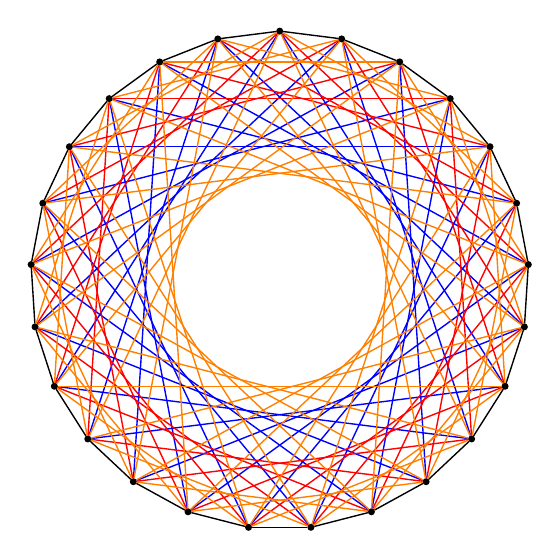
\begin{tikzpicture}[scale=.6]


\GraphInit[vstyle=Simple]
\tikzset{VertexStyle/.append style = {minimum size =2pt, inner sep = 0pt}}


\Vertex[x=187.5pt,y=337.5pt]{0};
\Vertex[x=224.80348307472823pt,y=332.7874741692947pt]{1};
\Vertex[x=259.7630511152573pt,y=318.94600200657953pt]{2};
\Vertex[x=290.1820658893033pt,y=296.8452941132117pt]{3};
\Vertex[x=314.14918882530225pt,y=267.87401924684946pt]{4};
\Vertex[x=330.15847744427305pt,y=233.85254915624213pt]{5};
\Vertex[x=337.2040092642407pt,y=196.91857792939703pt]{6};
\Vertex[x=334.8430876093033pt,y=159.3928028121413pt]{7};
\Vertex[x=323.22405786990294pt,y=123.63310626523908pt]{8};
\Vertex[x=303.0769864163684pt,y=91.88640153769651pt]{9};
\Vertex[x=275.667787843871pt,y=66.14745084375791pt]{10};
\Vertex[x=242.71868290270174pt,y=48.0335271167623pt]{11};
\Vertex[x=206.2999850346457pt,y=38.682794802828326pt]{12};
\Vertex[x=168.70001496535434pt,y=38.682794802828326pt]{13};
\Vertex[x=132.2813170972983pt,y=48.03352711676226pt]{14};
\Vertex[x=99.3322121561291pt,y=66.14745084375782pt]{15};
\Vertex[x=71.92301358363159pt,y=91.88640153769656pt]{16};
\Vertex[x=51.77594213009703pt,y=123.63310626523916pt]{17};
\Vertex[x=40.1569123906967pt,y=159.3928028121413pt]{18};
\Vertex[x=37.795990735759275pt,y=196.91857792939695pt]{19};
\Vertex[x=44.841522555726954pt,y=233.8525491562421pt]{20};
\Vertex[x=60.85081117469775pt,y=267.8740192468495pt]{21};
\Vertex[x=84.81793411069665pt,y=296.8452941132117pt]{22};
\Vertex[x=115.23694888474257pt,y=318.9460020065795pt]{23};
\Vertex[x=150.1965169252717pt,y=332.7874741692946pt]{24};

\SetUpEdge[lw         = .5pt,
            color      = black,
            labelcolor = black]

\Edge(24)(0)
\Edge(0)(1)
\Edge(1)(2)
\Edge(2)(3)
\Edge(3)(4)
\Edge(4)(5)
\Edge(5)(6)
\Edge(6)(7)
\Edge(7)(8)
\Edge(8)(9)
\Edge(9)(10)
\Edge(10)(11)
\Edge(11)(12)
\Edge(12)(13)
\Edge(13)(14)
\Edge(14)(15)
\Edge(15)(16)
\Edge(16)(17)
\Edge(17)(18)
\Edge(18)(19)
\Edge(19)(20)
\Edge(20)(21)
\Edge(21)(22)
\Edge(22)(23)
\Edge(23)(24)

\SetUpEdge[lw         = .5pt,
            color      =blue,
            labelcolor = black]

\Edge(0)(8)
\Edge(2)(10)
\Edge(4)(12)
\Edge(6)(14)
\Edge(8)(16)
\Edge(10)(18)
\Edge(12)(20)
\Edge(14)(22)
\Edge(16)(24)
\Edge(18)(1)
\Edge(20)(3)
\Edge(22)(5)
\Edge(24)(7)
\Edge(1)(9)
\Edge(3)(11)
\Edge(5)(13)
\Edge(7)(15)
\Edge(9)(17)
\Edge(11)(19)
\Edge(13)(21)
\Edge(15)(23)
\Edge(17)(0)
\Edge(19)(2)
\Edge(21)(4)
\Edge(23)(6)

\SetUpEdge[lw         = .5pt,
            color      =red,
            labelcolor = black]

\Edge(0)(6)
\Edge(6)(12)
\Edge(12)(18)
\Edge(18)(24)
\Edge(24)(5)
\Edge(5)(11)
\Edge(11)(17)
\Edge(17)(23)
\Edge(23)(4)
\Edge(4)(10)
\Edge(10)(16)
\Edge(16)(22)
\Edge(22)(3)
\Edge(3)(9)
\Edge(9)(15)
\Edge(15)(21)
\Edge(21)(2)
\Edge(2)(8)
\Edge(8)(14)
\Edge(14)(20)
\Edge(20)(1)
\Edge(1)(7)
\Edge(7)(13)
\Edge(13)(19)
\Edge(19)(0)

\SetUpEdge[lw         = .5pt,
            color      =orange,
            labelcolor = black]

\Edge(0)(4)
\Edge(4)(8)
\Edge(8)(12)
\Edge(12)(16)
\Edge(16)(20)
\Edge(20)(24)
\Edge(24)(3)
\Edge(3)(7)
\Edge(7)(11)
\Edge(11)(15)
\Edge(15)(19)
\Edge(19)(23)
\Edge(23)(2)
\Edge(2)(6)
\Edge(6)(10)
\Edge(10)(14)
\Edge(14)(18)
\Edge(18)(22)
\Edge(22)(1)
\Edge(1)(5)
\Edge(5)(9)
\Edge(9)(13)
\Edge(13)(17)
\Edge(17)(21)
\Edge(21)(0)
\Edge(0)(9)
\Edge(9)(18)
\Edge(18)(2)
\Edge(2)(11)
\Edge(11)(20)
\Edge(20)(4)
\Edge(4)(13)
\Edge(13)(22)
\Edge(22)(6)
\Edge(6)(15)
\Edge(15)(24)
\Edge(24)(8)
\Edge(8)(17)
\Edge(17)(1)
\Edge(1)(10)
\Edge(10)(19)
\Edge(19)(3)
\Edge(3)(12)
\Edge(12)(21)
\Edge(21)(5)
\Edge(5)(14)
\Edge(14)(23)
\Edge(23)(7)
\Edge(7)(16)
\Edge(16)(0)

\end{tikzpicture}
\end{center}



\begin{itemize}
		\item<1->
\begin{center}
Cay($\mathbb{Z}_{25}$, \{$\pm$1,$\pm$4,$\pm$6,$\pm$8\})     
\end{center}
                 
\end{itemize}
}



\frame {
	\frametitle{\underline{Introduction to Cayley Graphs}}
	\only<1>{
	\begin{itemize}
                  \item<1-> Definition:  Let $\Gamma$ be a finite group with a subset A. The \underline{\emph{Cayley digraph}}, denoted Cay($\Gamma$,A), is a digraph with vertex set $\Gamma$, such that (x,y) is a directed edge if and only if $yx^{-1}$ $\in$ A

		\item<1->\emph{Cayley digraphs} are vertex transitive.


	\end{itemize}
}
}


\frame{

\frametitle{\underline{Introduction to Cayley Graphs}}

\begin{itemize}
		\item<1->

The bicycle wheel

\end{itemize}

\begin{center}
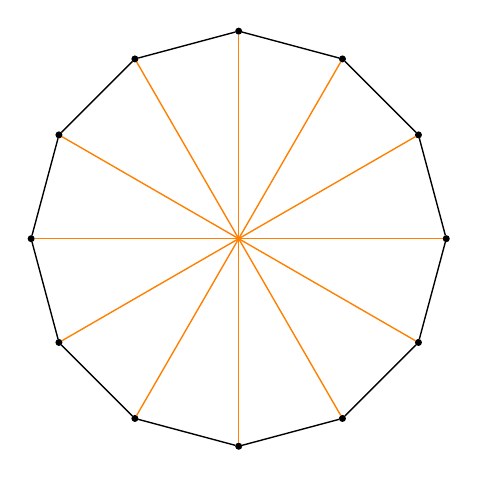
\begin{tikzpicture}[scale=.5]


\GraphInit[vstyle=Simple]
\tikzset{VertexStyle/.append style = {minimum size =2pt, inner sep = 0pt}}


\Vertex[x=187.5pt,y=337.5pt]{0};
\Vertex[x=262.5pt,y=317.4038105676658pt]{1};
\Vertex[x=317.4038105676658pt,y=262.5pt]{2};
\Vertex[x=337.5pt,y=187.5pt]{3};
\Vertex[x=317.4038105676658pt,y=112.50000000000004pt]{4};
\Vertex[x=262.5pt,y=57.596189432334185pt]{5};
\Vertex[x=187.50000000000003pt,y=37.5pt]{6};
\Vertex[x=112.50000000000004pt,y=57.596189432334185pt]{7};
\Vertex[x=57.59618943233425pt,y=112.49999999999991pt]{8};
\Vertex[x=37.5pt,y=187.49999999999997pt]{9};
\Vertex[x=57.59618943233421pt,y=262.5pt]{10};
\Vertex[x=112.49999999999994pt,y=317.4038105676658pt]{11};


\SetUpEdge[lw         = .5pt,
            color      =black,
            labelcolor = black]
\Edge(0)(1)
\Edge(1)(2)
\Edge(2)(3)
\Edge(3)(4)
\Edge(4)(5)
\Edge(5)(6)
\Edge(6)(7)
\Edge(7)(8)
\Edge(8)(9)
\Edge(9)(10)
\Edge(10)(11)
\Edge(11)(0)

\SetUpEdge[lw         = .5pt,
            color      =orange,
            labelcolor = black]

\Edge(0)(6)
\Edge(9)(3)
\Edge(2)(8)
\Edge(7)(1)
\Edge(11)(5)
\Edge(10)(4)

\end{tikzpicture}
\end{center}


\begin{center}
Cay($\mathbb{Z}_{12}$, \{$\pm$1,$\pm$6,\})     
\end{center}



}


\frame{
\frametitle{\underline{Introduction to Cayley Graphs}}

\begin{itemize}
		\item<1->  The Petersen Graph

\end{itemize}

\begin{center}
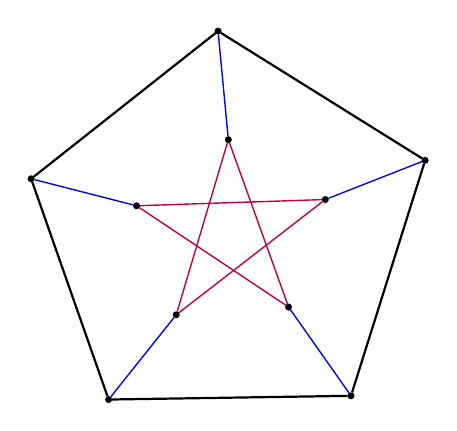
\begin{tikzpicture}[scale=.6]


\GraphInit[vstyle=Simple]
\tikzset{VertexStyle/.append style = {minimum size =2pt, inner sep = 0pt}}

\Vertex[x=76.42941276749721pt,y=222.11672788567688pt]{0};
\Vertex[x=188.99428167091503pt,y=311.04722529413755pt]{1};
\Vertex[x=313.69705213095506pt,y=233.22858659510686pt]{2};
\Vertex[x=269.05636402340275pt,y=91.41442753601768pt]{3};
\Vertex[x=123.08023124502833pt,y=89.1708736174299pt]{4};
\Vertex[x=139.9280102908217pt,y=205.8448415441469pt]{5};
\Vertex[x=195.1737949263097pt,y=245.68890432812992pt]{6};
\Vertex[x=253.59353344956895pt,y=209.6206717576203pt]{7};
\Vertex[x=231.46826299919053pt,y=144.8606369231964pt]{8};
\Vertex[x=163.80751418745828pt,y=140.21907743256966pt]{9};

\Edge(0)(1)
\Edge(1)(2)
\Edge(2)(3)
\Edge(4)(0)
\Edge(4)(3)

\SetUpEdge[lw         = .5pt,
            color      =purple,
            labelcolor = black]
\Edge(5)(7)
\Edge(7)(9)
\Edge(9)(6)
\Edge(6)(8)
\Edge(8)(5)


\SetUpEdge[lw         = .5pt,
            color      =blue,
            labelcolor = black]

\Edge(9)(4)
\Edge(0)(5)
\Edge(1)(6)
\Edge(7)(2)
\Edge(3)(8)



\end{tikzpicture}


\end{center}

\begin{itemize}
		\item<1->
\begin{center}
This is not a Cayley digraph. 
\end{center}
                 
\end{itemize}

}

\frame{
	\frametitle{\underline{N-Cubes}}
\begin{itemize}
\item<1-> \underline{Definition}: The Cayley digraph Cay($\Z_2^n$, \{$e_1$, $e_2$, ... , $e_n\}$)
\item<1-> Common choice for interconnection network designs
 \item<1-> The diameter of a network represents the maximum communication delay between two nodes in the network. 
               \item<1-> For a fixed diameter and vertex degree, there are circulant graphs that contain more vertices than the corresponding n-cube.
 \item<1-> Hence, circulant graphs give better communication networks than cubes
\end{itemize}

}


\frame{
\frametitle{\underline{N-Cubes}}

\begin{itemize}
		\item<1->  The 3-Cube

\end{itemize}

\begin{center}

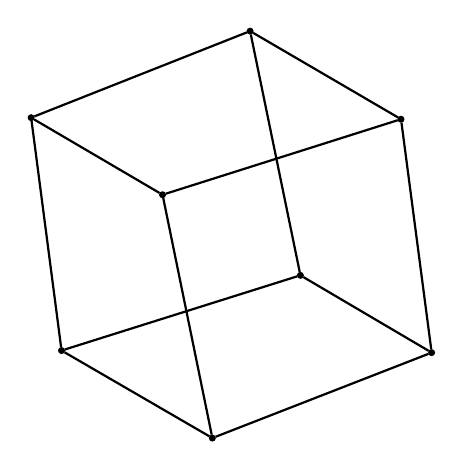
\begin{tikzpicture}[scale=.8]


\GraphInit[vstyle=Simple]
\tikzset{VertexStyle/.append style = {minimum size =2pt, inner sep = 0pt}}

\Vertex[x=110.02862790300208pt,y=131.87672511866043pt]{0};
\Vertex[x=96.30215571622227pt,y=237.05155446176758pt]{1};
\Vertex[x=217.91321401104452pt,y=165.84697363526885pt]{2};
\Vertex[x=195.20255762041074pt,y=276.1568088613707pt]{3};
\Vertex[x=178.15328202069801pt,y=92.3523239240585pt]{4};
\Vertex[x=155.65806918738338pt,y=202.2468746629973pt]{5};
\Vertex[x=277.20023675235643pt,y=130.94281761218554pt]{6};
\Vertex[x=263.36068740090917pt,y=236.3676312568985pt]{7};

\Edge(0)(1)
\Edge(1)(3)
\Edge(3)(2)
\Edge(2)(0)
\Edge(4)(5)
\Edge(5)(7)
\Edge(7)(6)
\Edge(6)(4)
\Edge(4)(0)
\Edge(5)(1)
\Edge(7)(3)
\Edge(6)(2)

\end{tikzpicture}

\end{center}


}

\frame {
	\only<1>{
	\begin{itemize}
                  \item<1-> For positive integers $d$ and $k$, we define:
\begin{align*}
m(d,A) &=\max\{m | diam(Cay(\mathbb{Z}_m,A)) \leq d\} \text{,} \\
m(d,k) &= \max_{A: |A| = k}\{m(d,A)  \}.
\end{align*}


	\end{itemize}
}



}

\frame{
	\only<1>{
	\begin{itemize}
                  \item<1-> Current known values include:
\begin{align*}
m(1,k) &= k+1,
\\
m(d,1) &= d+1\text{, and}
\\
m(d,2) &= \left\lfloor \frac{d(d+4)}{3} \right\rfloor+1 \text{ for all } d\geq2.
\end{align*}

	\end{itemize}
}
}






\frame{

The following theorem can be used to construct large efficient generating sets $A$  so that $m(d,A)$
is large by using small efficient generating sets.

\begin{theorem} \label{thm:addition.theorem.for.m(d,k)}
Let $d_1\ge2$, $d_2\ge2$, $k_1\ge1$, and $k_2\ge1$ be integers.  Then
\[
m(d_{1}+d_{2},k_1+k_2)\ge m(d_1,k_1)m(d_2,k_2).
\]
\end{theorem}

}

\frame{
\underline{Proof}\\
 Let 
$A_s=\{0<a_{s1}<a_{s2}<\cdots<a_{sk_s}\}$ be a set of integers with
\[
m(d_s,A_s)=m(d_s,k_s)=m_s\qquad\hbox{for}\quad s=1,2.
\]
We may assume, without loss of generality, that $a_{sk_{s}}<m_{s}$ for $s=1,2$.
Define
\[
A=A_1\cup\{m_1a_{2j}\ |\ j=1,2,\ldots,k_2\}.
\]
Since $|A|=k_1+k_2$, we only need to prove that $A$ is a $(d_1+d_2)$-basis for $\Z_{m_1m_2}$.


}

\frame
{
 Let $n$ be any nonnegative integer. Since $A_1$ is an $d_{1}$-basis for $\Z_{m_1}$, we see that
\[
n\equiv \sum_{i=1}^{k_1}x_{i}a_{1i}\pmod{m_1},
\]
where $x_{i}$'s are nonnegative integers with  $\ddd\sum_{i=1}^{k_{1}}x_{i}\le d_{1}$.  Assume
\[
n=\sum_{i=1}^{k_1}x_{i}a_{1i}+qm_1
\]
for some integer $q$.

}
\frame
{
 It follows from the fact that $A_2$ is a
$d_{2}$-basis for $\Z_{m_2}$ that
\[
q=\sum_{j=1}^{k_2}y_{j}a_{2j}+pm_2,
\]
where $y_{j}$'s are nonnegative integers with  $\ddd\sum_{j=1}^{k_{2}}y_{j}\le d_{2}$, and $p$ is an integer.

}

\frame
{
 Therefore,
\[
n\equiv\sum_{i=1}^{k_1}x_{i}a_{1i}+\sum_{j=1}^{k_2}y_{j}m_1a_{2j}\pmod{m_1m_2},
\]
where
\[
\sum_{i=1}^{k_{1}}x_{i}+\sum_{j=1}^{k_{2}}y_{j}\le d_{1}+d_{2}.
\]
This implies that $n\in (d_1+d_2)A_{0}$, where $A_{0}=A\cup\{0\}$. Hence, $A$ is a $(d_{1}+d_{2})$-basis for $\Z_{m_1m_2}$. Therefore,
\[
m(d_{1},k_{1})m(d_{2},k_{2})=m_{1}m_{2}\le m(d_{1}+d_{2},k_{1}+k_{2}).
\]
The proof is complete.

}

\frame
{
\frametitle{\underline{The General Case}}
\only<1> 
\begin{itemize}
\item<1->By repeated application of this inequality, and using lower bounds for small values of k
we can construct a bound for general k 

\end{itemize}

}

\frame{
\frametitle{\underline{Computability of m(d,k)}}
Let $d$ be the diameter for $\Cay(m, k)$.
\\ 
Given $d$ define fixed $d_{1}$ to be $\frac{d}{\lambda}$, also define $a_{1} = \frac{a}{\lambda}$, $b_{1} = \frac{b}{\lambda}$, and $c_{1} = \frac{c}{\lambda b}$, etc.., so $\lambda$ is a large number determined by $d$. The parameter $\lambda$ will not appear in the code, but it enables us to compute a lower bound as a function of $d$.
}
\frame{

\frametitle{\underline{Computability of m(d,k) for small fixed k}}
Our lower bound on $m(d, k)$ will be defined as $m =\alpha \lambda a_{1} + \beta \lambda b_{1} + \gamma \lambda c_{1}$+ ... $\psi \lambda z_{1}$.  To determine the validity of the lower bound, we compute every point in $dA$ as a polynomial in terms of $\lambda$.


%%\\ \\
%%For notational simplicity, we will denote $a_{1}$, $b_{1}$ and $c_{1}$ as $a, b$ and $c$.
%\\ \\
%%To check that a given polynomial bound is correct, we 
%%$\forall$  $\mathcal{A}$ = $\{(a,  b,  c, ... ,  z)  \vert  (\alpha  a, \beta  b, \gamma  c, .. , \psi  z) \} \subseteq \mathbb{Z}_{m}$, find $\mathbb{Z}_{m}$ with the largest cardinality such that $dA \cong \mathbb{Z}_{m}$.


}

\frame
{
\frametitle{\underline{Computability of m(d,k) for small fixed k}}
Take ($x_{1}, x_{2}, ... , x_{n}$) such that $x_{1} \leq b_{1}, x_{2} \leq c_{1}, .. , x_{n} \leq \psi$ and $\sum_{i} x_{i} \leq d$ %%t$, where $t$ represents the number of cycles needed by each generating set to complete a covering of $\mathbb{Z}_{m}$.
\\
For all polynomials $x_{1}a + x_{2}b + .. + x_{n}k$, we reduce to a unique minimal representation by comparing the coefficients $(x_{1}, x_{2}, x_{3}, .. , x_{n})$ and $(\alpha, \beta, \gamma, .. , \psi)$ and removing dependent linear combinations.
}
\frame{
\frametitle{\underline{Computability of m(d,k) for small fixed k}}
$\forall x = (x_{1}, x_{2}, .. , x_{k}) \in dA$ if $x \notin \mathbb{Z}_m$, we can identify $x$ with point $x' = (x'_{1}, x'_{2}, .. , x'_{k}) \in \mathbb{Z}_{m}$ congruent to $x$ $(mod$ $m)$.  Then if every point $n \in \mathbb{Z}_{m}$ is either equal to some $x$ or $x'$, $dA = \mathbb{Z}_m$. 
\\ 
To construct a lower bound, we systematically check combinations of generators $A$ and coefficients, and record the largest $m$ (and corresponding generators) such that a covering by $dA$ is achieved.
}

\end{document}